\documentclass[12pt]{article}
\title{\vspace{-2.5cm}\Large{Do Homeowners Care About Air Quality? Estimating the Effect of Poor Air Quality on Home Prices Using Wildfire Smoke Data}} 
\author{\normalsize Tristan Misko}
\date{\normalsize{17 December 2021}}

\usepackage{amsmath}
\usepackage{amsfonts}
\usepackage{mathrsfs}
\usepackage{amssymb}
\usepackage{yfonts}
\usepackage{bbm}
\usepackage{graphics}
\usepackage[margin=1 in]{geometry}

\let\biconditional\longleftrightarrow
\let\iff\Leftrightarrow
\let\implies\Rightarrow
\let\infinity\infty
\let\by\times
\let\iso\cong
\let\unif\rightrightarrows
\DeclareRobustCommand{\Z}{\mathbb Z}
\DeclareRobustCommand{\hom}{\text{Hom}\,(\Z,G)}
\DeclareRobustCommand{\N}{\mathbb N}
\DeclareRobustCommand{\R}{\mathbb R}
\DeclareRobustCommand{\C}{\mathbb C}
\DeclareRobustCommand{\Q}{\mathbb Q}
\DeclareRobustCommand{\E}{\mathbb E}
\DeclareRobustCommand{\P}{\mathbb P}
\DeclareRobustCommand{\tr}{\text{tr}}
\DeclareRobustCommand{\norm}{\mathrel{\unlhd}}
\DeclareRobustCommand{\contains}{\supset}
\DeclareRobustCommand{\lcm}{\text{lcm}}
\DeclareRobustCommand{\glnr}{GL(n,\R)}
\DeclareRobustCommand{\limit}{\lim_{n\to\infinity}}
\DeclareRobustCommand{\nti}{{n\to\infinity}}
\DeclareRobustCommand{\del}{\partial}
\DeclareRobustCommand{\graph}{\text{graph}\,}
\DeclareRobustCommand{\interior}{\text{int}\,}
\DeclareRobustCommand{\Var}{\text{Var}}
\DeclareRobustCommand{\Cov}{\text{Cov}}
\DeclareRobustCommand{\normal}{\mathcal N}
\DeclareRobustCommand{\Bar}{\overline}

\usepackage{titlesec}
\titleformat*{\section}{\normalsize\bfseries}
\titleformat*{\subsection}{\normalsize\bfseries}
\titleformat*{\subsubsection}{\normalsize\bfseries}
\titleformat*{\paragraph}{\normalsize\bfseries}
\titleformat*{\subparagraph}{\large\bfseries}

\usepackage{mathtools}
\DeclarePairedDelimiter\ceil{\lceil}{\rceil}
\DeclarePairedDelimiter\floor{\lfloor}{\rfloor}
\usepackage{cancel}

\usepackage{pgfplots}
\usepackage{tikz}
\usetikzlibrary{patterns}
\usetikzlibrary{calc}
\usepgfplotslibrary{polar}

\usepackage[english]{babel}
\usepackage[utf8]{inputenc}
\usepackage{multicol}
\usepackage{fancyhdr}

\pagestyle{fancy}
\fancyhf{}
\lhead{Tristan Misko}
\rhead{\small{ECON 191}}
\cfoot{\thepage}

\usepackage{mathrsfs}
\usepackage{multirow}
\usepackage{hyperref}
\usepackage{textcomp}
\usepackage{xcolor}
\usepackage{setspace}

\usepackage{listings}
\usepackage{color}

\definecolor{dkgreen}{rgb}{0,0.6,0}
\definecolor{gray}{rgb}{0.5,0.5,0.5}
\definecolor{mauve}{rgb}{0.58,0,0.82}

\lstset{frame=tb,
  language=R,
  aboveskip=3mm,
  belowskip=3mm,
  showstringspaces=false,
  columns=flexible,
  basicstyle={\small\ttfamily},
  numbers=none,
  numberstyle=\tiny\color{gray},
  keywordstyle=\color{blue},
  commentstyle=\color{dkgreen},
  stringstyle=\color{mauve},
  breaklines=true,
  breakatwhitespace=true,
  tabsize=4
}

\begin{document}
	\maketitle
	\doublespacing
	
\section{Introduction} 

Economists have long understood housing prices as a hedonic function of various amenities offered by a housing unit and its surroundings.  These amenities take many forms, including among them employment opportunities, neighborhood characteristics, cultural amenities, local school quality, proximity to friends and family, idiosyncratic locational preferences, 
and environmental amenities.   Hedonic modeling allows us to infer the market valuation of non-market goods like environmental amenities from market prices, yielding important information about preferences and valuations that are difficult to see directly from market values.

In this paper, we explore the value that homeowners place on air quality by estimating the causal effect of declines in air quality due to wildfire increased smoke exposure.  Wildfire smoke contains a number of pollutants, most salient for health outcomes is PM 2.5 (EPA).  Chronic exposure to PM 2.5 can lead to significant declines in life expectancy, on the order of -0.35 years for a 10 $\mu g/m^3$ reduction in particulate matter (Apte).  

Under the logic of a hedonic model, homebuyers are sophisticated agents who take into account these potentially significant effects of air quality on life expectancy and health outcomes among all other factors, suggesting a potentially large effect of air quality on housing prices.  On the other hand, the consequences of living amid chronic air quality are temporally delayed and difficult to quantify, so homeowners may not be considering these effects fully when choosing housing.  Moreover, the market for clean air may also suffer from information problems, since light pollution is not often visible directly to homeowners who do not seek out AQI information directly.  


\section{Relationship to the Literature}

This paper attempts to contribute to the existing literature on estimating the causal effect of multi-year air quality shocks on housing prices, and explores the concept of thresholding nonlinearities in preferences about housing prices.  In particular, it may be that homeowners do not respond to air quality inside a certain band of acceptability, but begin to respond once the air quality moves outside that band.

A 2005 paper by Chay and Greenstone uses a spatial hedonic approach based on a United States Clean Air Act policy which implemented stricter regulations on counties which failed to meet pre-specified particulate pollution targets.  They estimate that a 1\% increase in particulate matter pollution concentration decreases home values by approximately 0.2\% to 0.35\% (Chay and Greenstone, 2005).  The fundamental idea of Chay and Greenstone's study is to use an instrument for air quality, namely non-attainment status under the Clean Air Act, to get plausibly exogenous variation in air quality; my strategy is similar in that wildfire smoke introduces plausibly exogenous variation in air quality that I will use in my estimation strategy.  My wildfire smoke instrument represents an improvement on the non-attainment status instrument for a few reasons.   Non-attainment status is a dummy, while wildfire smoke is a continuously valued variable, which offers more variability to exploit in estimation of coefficients.  Furthermore, one must treat selection bias arguments very seriously in the non-attainment case: perhaps there are systematic unobserved factors which simultaneously affect whether a county is a non-attainment county and which also affect housing quality, potentially introducing omitted variables bias.  Wildfire smoke, treatment by which is largely determined by wind patterns, admits fewer compelling arguments of this nature.

Kim et al. use a spatial hedonic approach at a very local level to estimate the effects of air pollution on housing prices in Seoul, South Korea, associating a 4\% air quality increase with a 1.4\% housing price increase (Kim et al., 2003).  They use a relatively small sample of households with detailed housing price data across all of the major districts of Seoul, controlling for neighborhood income and housing characteristic factors, along with a spatially interpolated local air pollution dataset.  Their estimates use spatially lagged variables as instruments, which is an econometric technique to overcome the lack of exogenous variation present in the cross-sectional price data but which is subject to many technical challenges (\textit{ibid}).  Zabel and Kiel employ a similar strategy in four U.S. cities, gathering data about individual housing units' prices and characteristics, controlling for neighborhood factors, and estimating a hedonic model for housing prices in Chicago, Denver, Philadelphia, and Washington D.C.  They find a small, significant negative relationship between air pollution and housing prices in two of them (Zabel and Kiel, 2000).  Instead of relying on sophisticated econometric techniques to overcome endogeneity in a cross-sectional sample as in both of these papers, my paper uses plausibly exogenous variation in air quality measured over multiple periods, which I believe is a stronger design.  My design applies to a more general setting than the estimates of these papers, which are city specific and may therefore lack the external validity that estimates generated from county-level data from across the U.S. would carry.   

Borgschulte et al. use wildfire smoke to instrument for air quality in their 2018 working paper estimating the causal effect of air quality on the labor market, particularly on employment and adaptation costs.  Although their outcome variable of interest is unrelated to housing prices, the machinery of their research design, which they claim is novel in their paper, is quite similar to the design I propose to use.  They use daily air quality data from the EPA, a wildfire smoke dataset based on satellite imagery to instrument for air quality, and identify their observations at the county level (Borgschulte et al., 2018).  Their paper is focused on estimating the effect of short term shocks of bad air quality on the labor market, which is different from my medium to long-run focus on housing prices as effected by changing trends in wildfire smoke.  

In summary, my paper can be understood as applying the research design using wildfire data similar to that deployed by Borgschulte et al. to the domain of housing prices.  Previous estimates of the causal effect of air quality housing prices have often been local, identified at the housing-unit level within a city or collection of cities, as in the cases of Kim et al. and Zabel and Kiel.  These estimates are clearly useful in the context of these cities, but they are open to external validity and generalizability critiques that my paper attempts to address by identifying observations across the United States at the county level.  The county-level identification of air quality and housing prices follows in the footsteps of Chay and Greenstone.  

\section{Data} 

The data take the form of panel data, with monthly observations at the US county level 
of the number of days in each month in which the county 
is covered by wildfire smoke plumes, the mean air quality index (AQI) over 
the month, and the level of the Zillow housing price index in that month.  
I also have associated to each observation a set of controls for
unemployment level and population density. 

\subsection{Wildfire Smoke}

The wildfire smoke data used in this paper was produced from an incredibly detailed dataset
put together by Vargo in 2019, which included daily satellite observations of light, 
medium, and heavy smoke plumes at the census block level (Vargo).  In order to use this data, a few important aggregation decisions were made:  

\begin{enumerate}
\item The smoke exposure ``dummy'' at the county level on a given day is a population-weighted continuous variable with values on $[0,1]$.  For example, suppose a county contains ten census blocks, three of which contain 50\% of the population of the county.  If these three blocks receive light smoke exposure on a given day, then the county level smoke exposure for that day is 0.5, the population weighted dummy for exposure in the county.  
\item In order to capture all of the smoke data in a single variable, we compute a weighted sum of the light smoke, medium smoke, and heavy smoke exposure variables for each day.  The weights in the sum follow from the NOAA definitions of smoke plume intensity, which tracks the density.\footnote{In particular, "Light" corresponds to $0-11\frac{\mu g}{m^3}$, "Medium" to $12-22\frac{\mu g}{m^3}$, and "Heavy" to $23^+\frac{\mu g}{m^3}$.  Weights of 6, 17, and 25, respectively, were used.}  Hence, the "smoke score" for each day approximately measures the total exposure to smoke in micrograms.  
\item Finally, we aggregate to the monthly level by summing daily scores over the months to obtain monthly estimates for smoke exposure.  
\end{enumerate}

The data exclude all counties in geographic west of the United States, as such 
counties may suffer from potentially significant confounding effects because 
wildfire events are heavily correlated with smoke events and may also affect housing prices.

\subsection{Zillow Home Value Index} The Zillow Home Value Index is a smoothed metric of housing prices which accounts.  It can be roughly interpreted as a smoothed dollar value for the 35th to 65th percentile of home values in a county (Zillow).  

\begin{singlespace}

\subsection{Variable Descriptions}

\begin{itemize}
\item $\text{price}_{c,t}$ (\textit{numeric variable}): The Zillow Home Value Index 
value, a smoothed indicator of housing prices in county $d$ and time period $t$.
\item $\text{smoke}_{c,t}$ (\textit{dummy variable}): A time-dependent treatment variable
determined from the smoke score, which a weighted sum of the number of light, medium
and heavy smoke days over the month within each county.  The dummy is one if we are in the
post treatment period (beginning 2015) and the county
experiences a change in mean monthly smoke score above a threshold value across the pre- and post-treatment period.
\item $D_c$ (\textit{dummy variable}): A set of dummy variables for the county fixed effects.  
\item $T_t$ (\textit{dummy variable}): A set of dummy variables for the time fixed  effects.
\item $\text{Unemp}_{c,g(t)}$ (\textit{numeric variable}): The quarterly unemployment rate at the county level.  Here, $g$ denotes the mapping of months to quarters.  
\item $HC_{c,t}$ (\textit{numeric variable}): A set of controls for the characteristics of the average home in a county
\item $\text{Density}_c$: The 2020 county density -- we assume that the density of counties are roughly constant over this period.
\end{itemize}
\end{singlespace}


\section{Models}

\subsection{Modeling Assumptions}

We argue that the wildfire smoke distribution is plausibly exogenous because it is governed by large scale flows in the atmosphere as well as local weather variations.  Because smoke plumes travel thousands of miles from East to West across the U.S., smoke exposure outside of the geographic West is generally unrelated to the factors which cause wildfires.  This produces a natural experiment setup in which some counties are treated with smoke while others are not, with variation in treatment status that is as good as random.   

In order to determine treatment status, we divide the period from 2010 to 2019 at a threshold month and compare the average in the before period to the average in the after period.  Because there is no hard threshold for when we can think of treatment turning on, we compare the coefficients estimated across five potential cutoff dates: December 2013, May 2014, December 2014, May 2015, and December 2015.  Although the graph does not show a drastic increase in wildfire smoke in the second part of the decade, there is a very change in the distribution of wildfire smoke across this period, with large swaths of the Eastern and Northern U.S. receiving large percentage increases in wildfire smoke.  

Below, we refer to the percentage change in mean smoke exposure between the interval of June 2010 to the treatment threshold and the interval from the treatment threshold to June 2019 as a \textbf{``medium run percentage change''} in wildfire smoke exposure for linguistic ease.  All use of this terminology in the paper refers to this specific definition. 

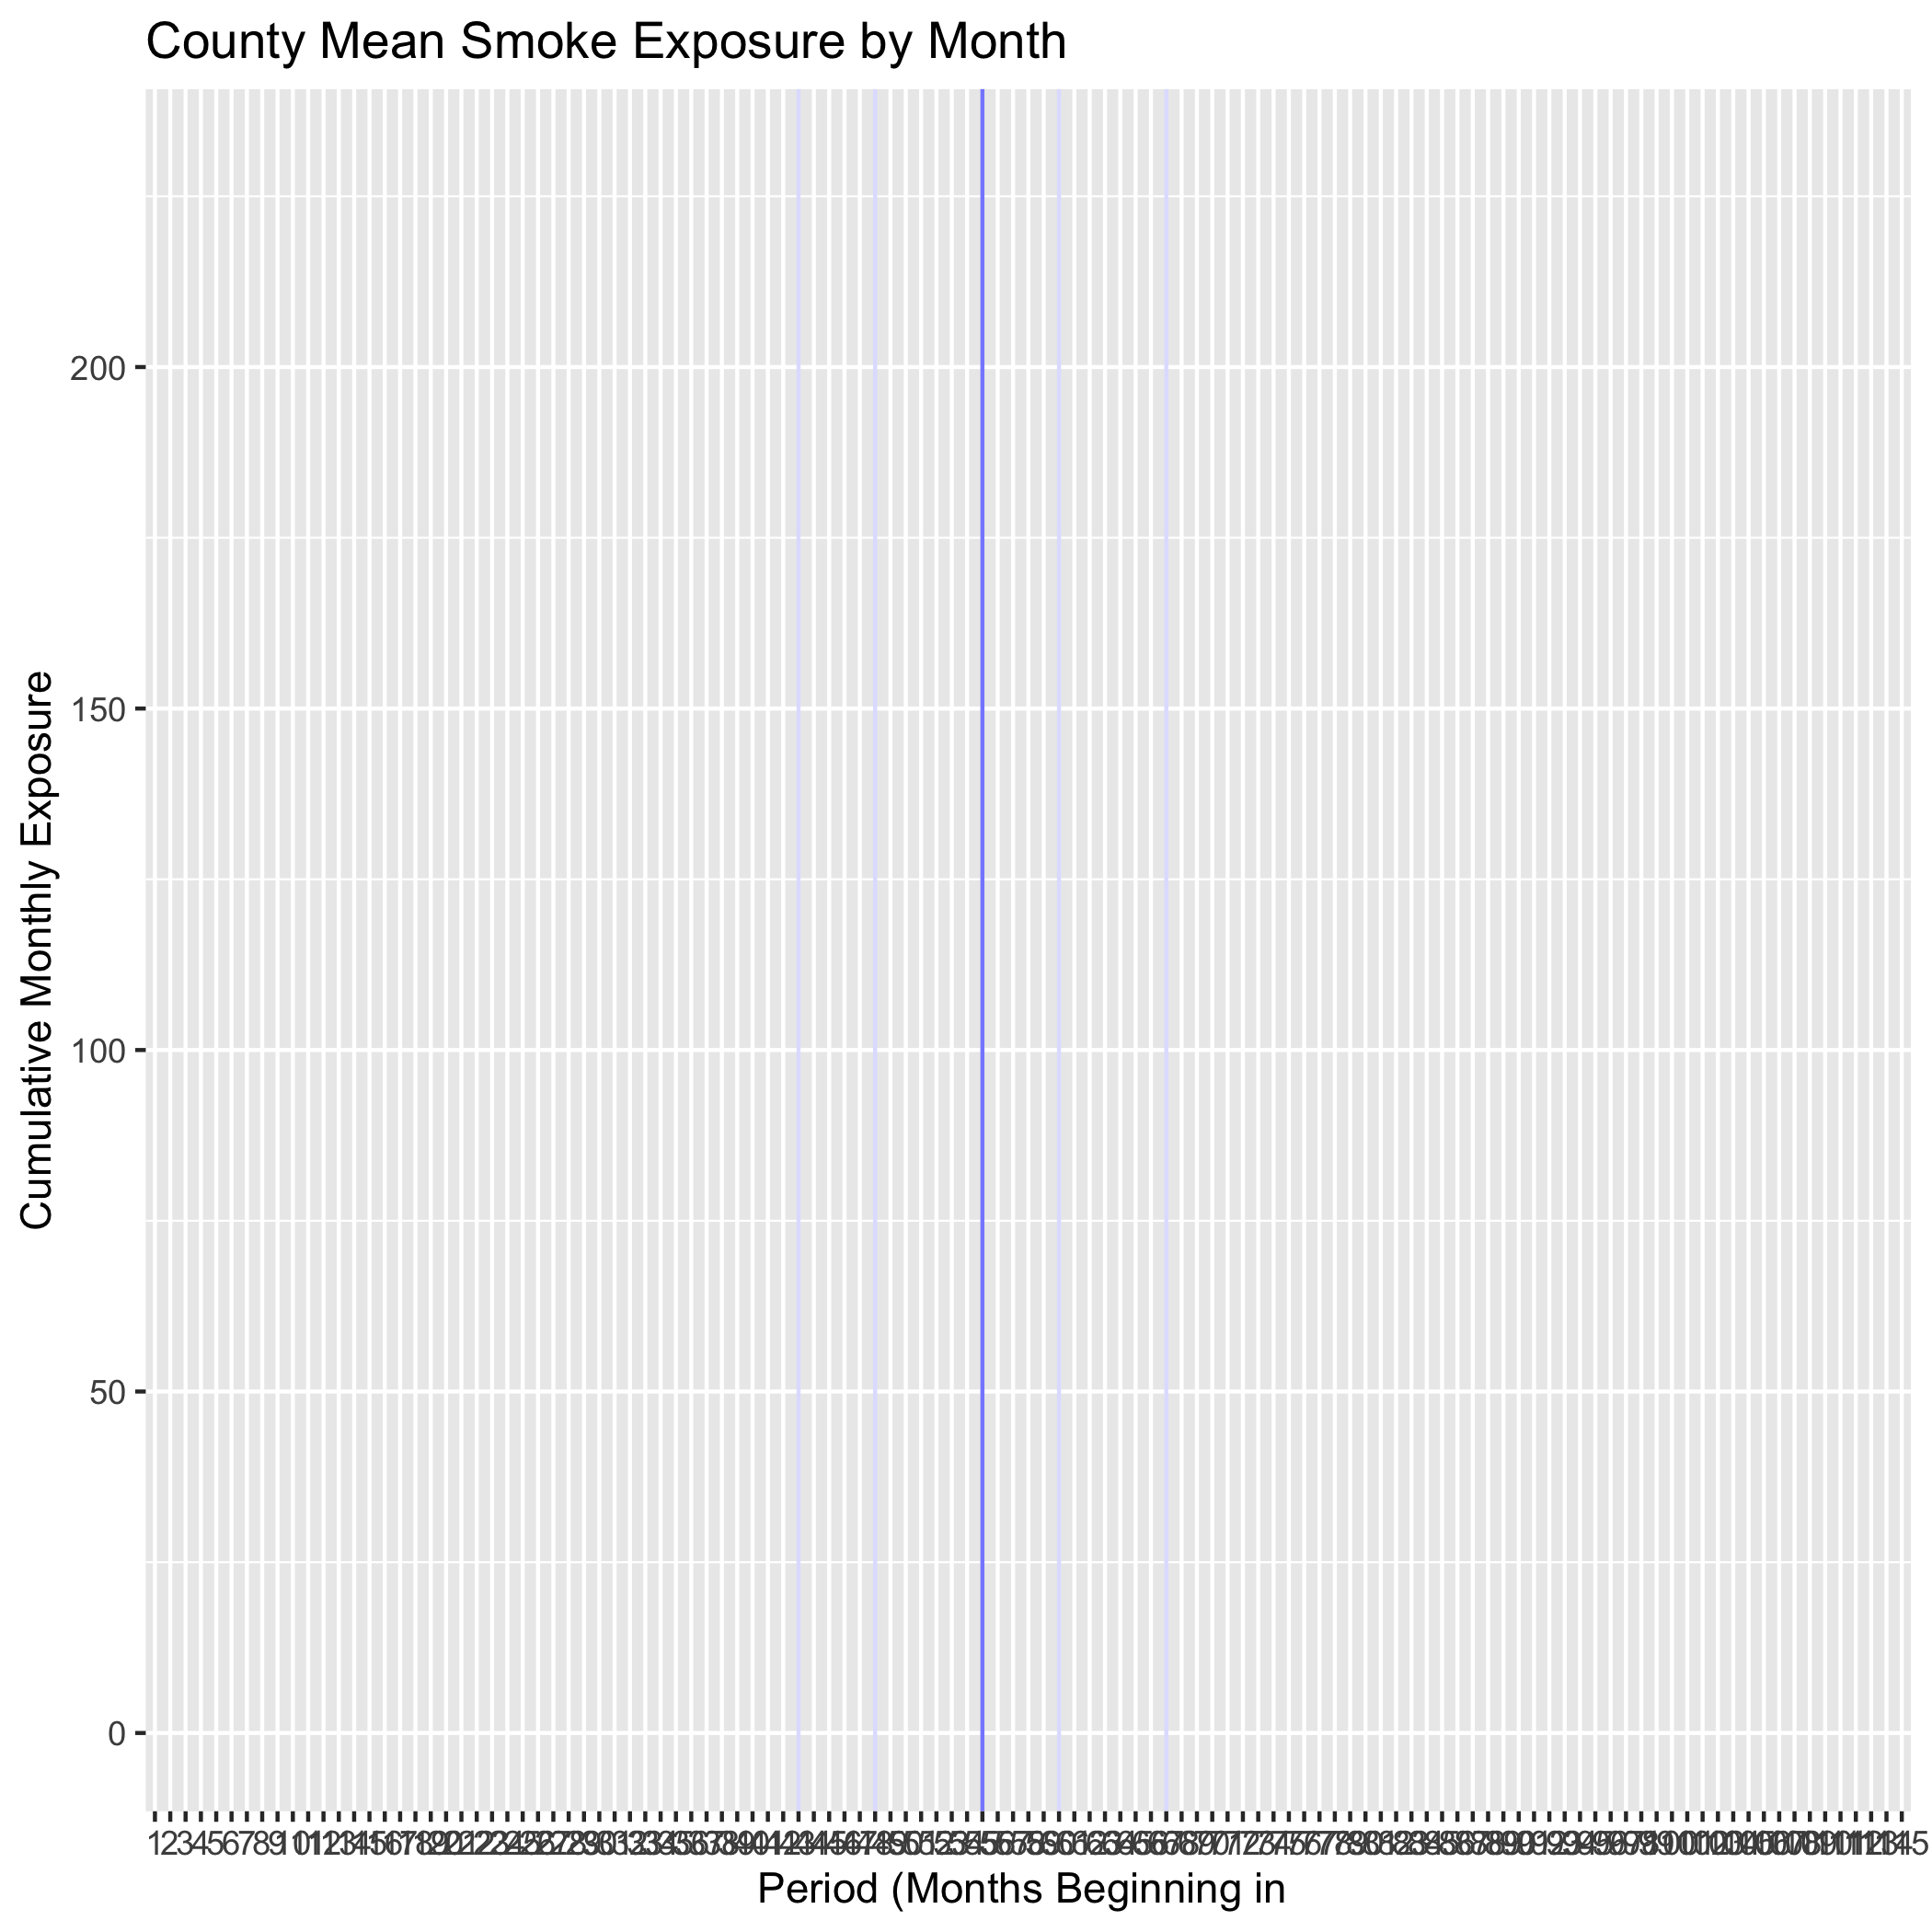
\includegraphics[scale = 0.6]{smoke_means}

\subsection{Model Specifications}

We model the effect of wildfire smoke on housing prices in a number of forms, allowing us to use different features of the variability in smoke exposure to estimate the causal effect of wildfire smoke under different modeling assumptions.  

We first estimate an OLS model with a number of controls given by
$$\text{ZHVI}_{c,t} = \beta_\text{OLS}\cdot \text{smoke}_{c,t} + \gamma\cdot \text{unemp}_{c,t} + \text{density}_c + T_t + \epsilon_{c,t},$$ running it both for $ZHVI_{c,t}$ and $\log(ZHVI)_{c,t}$ to look at level and percentage effects.  In this context, we interpret $\beta_\text{OLS}$ as the effect of a 1 $\frac{\mu g}{m^3}$ increase in wildfire smoke exposure on housing prices.  This regression does not exploit the random variability in the distribution of wildfire smoke, so it is not to be interpreted as a causal estimate, just as a correlation.  

We next estimate a similar model, but instead of using the monthly smoke exposure, we estimate the equation with the medium run percentage change in smoke percentage change.  

$$\text{ZHVI}_{c,t} = \beta_\text{OLS}\cdot \Delta\text{smoke}^{(t^* = 60)}_{c,t} + \gamma\cdot \text{unemp}_{c,t} + \delta\cdot\text{density}_c + T_t + \epsilon_{c,t}.$$

Estimating this equation also does not yield causal estimates, but it gives the corresponding correlational estimate for the effect of a change in the multiyear average.

Next, we run our main regression of interest, the treatment/control group regression given by 
$$\text{ZHVI}_{c,t} = \beta\cdot \text{smoke\_treatment}^{(t^* = 60)}_{c,t} + \gamma\cdot \text{unemp}_{c,t} + \delta\cdot\text{density}_c + F_c + T_t + \epsilon_{c,t}.$$
The dummy $\text{smoke\_treatment}^{(t^* = 60)}_{c,t}$ turns on if $t>60$, 
corresponding to the months following January 2015 and later, and if county $c$ is 
in the treatment group.  To characterize treatment status, we choose threshold values
for the percentage change in smoke score across the pre- and post-treatment 
periods.  The threshold values we select are arbitrary, therefore all results must
be carefully analyzed for sensitivity and robustness (see below).  For the main
regression, we characterize a county as "treated positive" if the increase in the
mean smoke score from the pre- to post-treatment period is greater than $50\%$, 
as "control" if the magnitude of the change in means is less than $5\%$, as 
"treated negative" if the decrease is greater than $50\%$ in magnitude, and as 
"boundary" otherwise.  

The final set of models which we estimate are those which have ``buckets'' for smoke
exposure corresponding to a percentage change of omitting the``boundary'' counties:
$$\text{ZHVI}_{c,t} = \left(\sum_{b} \beta_b\cdot B_b^{(t^* = 60)}\right) + \gamma\cdot \text{unemp}_{c,t} + \delta\cdot\text{density}_c + F_c + T_t + \epsilon_{c,t}.$$  Here, we allow more flexibility by letting the difference-in-differences coefficient depend on the treatment level.  Moreover, this specification allows us to look at potential threshold values: we expect the coefficient to be approximately zero near zero, and we can measure thresholding behavior by examining how wide the band is wherein the coefficients remain near zero.

\section{Main Results}

\subsection{OLS Model} The base OLS regression results are in line with what we would expect from our priors.  We detect a somewhat sizable negative relationship, with increase of one microgram per meter squared of exposure per month associated with a \$138.91 decline in housing values as measured by ZVHI, or alternatively, a 0.1\% decline in housing prices.  

The second set of OLS models has a coefficient which can be interpreted as a 1\% increase in medium run percentage change in smoke exposure is associated with a \$310.85 \textit{increase} in housing prices.  This has a perverse sign to what we would expect when thinking about air quality as a good people are willing to pay for.  Exploring the figures used in the analysis of the buckets models shows that the areas which received the largest increases in smoke exposure, mainly the geographic northeast, also happen to be more expensive, so this effect is certainly not causal and can be easily explained by spurious correlation.  

\begin{table}[!htbp] \centering 
  \caption{OLS Results} 
  \label{} 
\begin{tabular}{@{\extracolsep{5pt}}lcccc} 
\\[-1.8ex]\hline 
\hline \\[-1.8ex] 
 & \multicolumn{4}{c}{\textit{Dependent variable:}} \\ 
\cline{2-5} 
\\[-1.8ex] & zhvi.score & logZHVI & zhvi.score & logZHVI \\ 
\\[-1.8ex] & (1) & (2) & (3) & (4)\\ 
\hline \\[-1.8ex] 
 n.score & $-$138.910$^{***}$ & $-$0.001$^{***}$ &  &  \\ 
  & (3.567) & (0.00002) &  &  \\ 
  & & & & \\ 
 m.s.pch60 &  &  & 31,084.830$^{***}$ & 0.209$^{***}$ \\ 
  &  &  & (351.238) & (0.002) \\ 
  & & & & \\ 
 unemp & $-$12,133.240$^{***}$ & $-$0.094$^{***}$ & $-$12,155.620$^{***}$ & $-$0.095$^{***}$ \\ 
  & (76.539) & (0.0005) & (75.170) & (0.0005) \\ 
  & & & & \\ 
 density & 37.048$^{***}$ & 0.0001$^{***}$ & 36.065$^{***}$ & 0.0001$^{***}$ \\ 
  & (0.166) & (0.00000) & (0.165) & (0.00000) \\ 
  & & & & \\ 
 Constant & 236,814.200$^{***}$ & 12.497$^{***}$ & 228,138.400$^{***}$ & 12.443$^{***}$ \\ 
  & (1,637.335) & (0.010) & (1,604.653) & (0.010) \\ 
  & & & & \\ 
\hline \\[-1.8ex] 
Observations & 247,825 & 247,825 & 247,825 & 247,825 \\ 
R$^{2}$ & 0.258 & 0.237 & 0.276 & 0.261 \\ 
\hline 
\hline \\[-1.8ex] 
\textit{Note:}  & \multicolumn{4}{r}{$^{*}$p$<$0.1; $^{**}$p$<$0.05; $^{***}$p$<$0.01} \\ 
\end{tabular} 
\end{table} 

\subsection{Treatment/Control Model} The treatment control model attempts to overcome the endogeneity by selecting a set of control counties (selected under the assumed good-as-random assignment of having an medium run smoke exposure percentage change less than some threshold) and a set of treatment counties (selected as higher than some threshold).  Although the model was run with county fixed effects, it appears that spatial autocorrelation within the treatment and control groups is responsible for the positive observed coefficient.  Examination of the map of treatment and control groups supports this hypothesis. From the map below, we can see how despite the randomized boundaries of the regions, they are largely connected and hence suffer from autocorrelation.

\begin{table}[!htbp] \centering 
  \caption{Treatment/Control Results} 
  \label{} 
\begin{tabular}{@{\extracolsep{5pt}}lcc}\\[-1.8ex] \\ \hline
Coefficient & Value & Standard Error \\  
\hline \\[-1.8ex]
(Intercept)    & 84997.9926   & (1192.2196) \\
treat.k5.t25  &   7048.6579   & (174.0785) \\
unemp        &   1507.4164    &  (40.8662) \\
(Intercept)   & 89832.5871  & (1418.2894) \\
treat.k5.t50 &  4981.8987  &  (206.1134) \\
unemp       &   1042.3432    &   (58.7912) \\
(Intercept)  &  166978.0474 & (1110.3854) \\
treat.k10.t25  &  6646.7527 &  (127.0532) \\
unemp         &   1410.9679  &  (35.5550) \\
(Intercept)  &  170480.2136 &   (1171.2642) \\
treat.k10.t50  &  4587.3365  &  (152.5765) \\
unemp         &    989.8005     &  (45.8351)  \\
\hline
\end{tabular}
\end{table}

\includegraphics[scale = 0.8]{tcmap}

\subsection{Buckets Model} We estimate the difference in differences bucket model described in the model section above.  We choose two specifications which divide up the counties into buckets with 10\% changes (here referred to as the Twenty One Buckets model) and the 20\% changes (here referred to as the Twelve Buckets Model).  For example, Bucket-3 in the Twenty One Buckets model includes all counties in the eastern United States which experienced a medium run percentage decrease in wildfire smoke of -30\% to -40\%.  This gives us multiple treatment groups each with a different treatment level.  One observation is that certain buckets contain very few counties, especially at the extremes, hence, inference from these groups is harder to justify.  

The results of the regressions are recorded in the tables below.  We can see that the unemployment and density controls have the correct sign and similar magnitude to that in the OLS version.   The coefficients on the buckets are more difficult to parse.  In the model we wrote down, these should represent the effect of a medium run smoke change in the range associated with each bucket on housing prices.  If the model were correctly capturing the causal effect, we would expect to see the effect be strongly positive for large decreases in the smoke exposure, strongly negative for the large increases in smoke exposure, and closer to zero as we approach zero from either end.  This pattern is most definitely not observed, and leads us to question the validity of the model.   



\begin{table}[!htbp] \centering 
  \caption{Twenty One Bucket Results} 
  \label{} 
\begin{tabular}{@{\extracolsep{5pt}}lcc}\\[-1.8ex] \\ \hline
Coefficient & Value & Standard Error \\  
\hline \\[-1.8ex]
(Intercept) & 229167.1007 & (1593.4667) \\
bucket-7  & 7579.4415$^{***}$   & (2120.9187) \\
bucket-6  & 12452.7418$^{***}$ & (1322.5544) \\
bucket-5  & -12753.8180$^{***}$ & (1197.0110) \\
bucket-4  & -40523.6278$^{***}$ & (1145.9454) \\
bucket-3  & -31501.3615$^{***}$ & (1119.2566) \\
bucket-2  & -45392.7693$^{***}$ & (1152.7616) \\
bucket-1  & -46298.2183$^{***}$ & (1116.4600) \\
bucket0   & -49104.0762$^{***}$ & (1016.8342) \\
bucket1   & -21775.0823$^{***}$ & (1050.0574) \\
bucket2   & -998.0032 & (991.8717) \\
bucket3   & -4714.8775$^{***}$ & (1017.3990) \\
bucket4   & -3.2480 & (1087.7196) \\
bucket5   & 18657.1179$^{***}$ & (2951.1417) \\ 
bucket6   & 6160.8812$^{***}$ & (1303.4413) \\ 
bucket7   &  17543.1939$^{***}$ & (1382.0056) \\
bucket8   &  -7915.7779$^{***}$ & (1742.4632) \\
bucket9   &  -13751.0039$^{***}$ & (1784.5302) \\
bucket10  &  -26182.7457$^{***}$ & (3613.4257) \\
bucket11  &   NA  &  NA \\
bucket12  &  41973.9373$^{***}$ & (3751.1691) \\
bucket13  &  43425.8995$^{***}$ & (6390.6147) \\
bucket14  &   NA  &  NA  \\
bucket15  &  27061.5994$^{***}$ & (8999.2158) \\
unemp     &   -11785.0877$^{***}$& (74.9822) \\
density   &       36.1491$^{***}$& (0.1647) \\
\hline
\end{tabular}
\end{table}


\begin{table}[!htbp] \centering 
  \caption{Twelve Bucket Model} 
  \label{} 
\begin{tabular}{@{\extracolsep{5pt}}lcc}\\[-1.8ex] \\
Coefficient & Value & Standard Error \\  
\hline \\[-1.8ex]
(Intercept) & 230009.7616$^{***}$ & (1597.6566) \\
bbucket-4  & -6109.1748$^{**}$ & (2816.4182) \\ 
bbucket-3 & -15963.0936$^{***}$ & (2170.0217) \\
bbucket-2 & -49418.9504$^{***}$ & (2132.6985) \\
bbucket-1 & -59533.4319$^{***}$ & (2137.8051) \\ 
bbucket0  & -50296.4293$^{***}$ & (2113.8585) \\
bbucket1  & -16378.6261$^{***}$ & (2107.8347) \\
bbucket2  & -13641.8188$^{***}$ & (2128.6999) \\
bbucket3  & -2330.2844$$ & (2192.0692) \\ 
bbucket4  & -24349.1420$^{***}$ & (2335.0775) \\
bbucket5  & -11080.8776$^{***}$ & (2710.7456) \\ 
bbucket6  &  28559.8834$^{***}$ & (3801.7263) \\
bbucket7  &  13223.2686$$ & (9228.9809) \\
unemp     & -11874.6629$^{***}$ & (75.0590) \\
density   &  36.0975   & (0.1644) \\
\end{tabular}
\end{table}

\includegraphics[scale = 0.7]{bucket_12}

\includegraphics[scale = 0.7]{bucket_21}

\section{Robustness Checks}

\subsection{Parallel Trends} We plot the mean ZHVI across the Treatment/Control
groups in each period and examine the evolution in time.  From the graph, it is
visually clear that the trends in the means are close to parallel, and it seems
that there is a small dip in the ZHVI for the treatment group after treatment.

For the buckets case, we plot the mean evolution in time within each bucket.  As we can see, the trends are not parallel in aggregate, although the majority of lines seems to follow a parallel trends pattern.  The outlier lines tend to be those with small sample sizes.  Because the parallel trends assumption fails in these circumstance, we can not make causal inference on the basis of this model.  The nonparallel trends may account to some extent for the significant coefficients which seem to show no clear pattern in the buckets model.

\includegraphics[scale = 0.7]{parallel_b}

\includegraphics[scale = 0.7]{parallel_bb}

\subsection{Percent Change Threshold for Treatment/Control Model:} Because we are selecting which counties are in the treatment group by setting the the threshold, it is crucial to analyze how sensitive the results are to our choice of threshold. In the figure we graph the coefficient output for $t^* = 60$ as a function of the selection threshold for inclusion in the treatment group.  We can see that as we contract the treatment group by making the percentage change required more restrictive, the coefficient drops down.  This makes some sense intuitively, for including only the counties which have the most extreme change in smoke should increase the negative effect.  It is worth noting that even with a very restrictive threshold, we still cannot overcome the spatial autocorrelation to get the negative estimate we expect.  

\includegraphics[scale = 0.7]{sense}

\subsection{Treatment Start Time:} We run the OLS and Treatment-Control models at the five different treatment periods mentioned above and compare the results in the table below. We can see that the results are indeed sensitive to the choice of time period, which casts further doubt on the validity of the model for causal inference.   

\begin{table}[!htbp] \centering 
  \caption{Treatment Start Time Sensitivities} 
  \label{} 
\begin{tabular}{@{\extracolsep{5pt}}lcc}\\[-1.8ex] \\
Coefficient & Value & Standard Error \\  
\hline \\[-1.8ex]
(Intercept)    & 98895.6742$^{***}$ & (923.2356) \\
treat.k10.t50 & -3507.9245$^{***}$ & (147.0831) \\
unemp           & 2191.4596$^{***}$ & (45.5383) \\
(Intercept)    &  92085.7062$^{***}$ &  (1427.3480)\\
treat.k10.t50 &   1546.4467$^{***}$ & (176.6525 )\\
unemp            & 805.2211$^{***}$ & (56.6808) \\
(Intercept)     & 102848.6906$^{***}$ & (956.3864)\\
treat.k10.t50   & -3673.3737$^{***}$ & (156.4296)\\
unemp            & 1592.4215$^{***}$ &  (38.3191) \\
(Intercept)    & 170480.2136$^{***}$ & (1171.2642) \\
treat.k10.t50   & 4587.3365$^{***}$ & (152.5765)\\
unemp           &  989.8005$^{***}$ & (45.8351) \\
(Intercept)   & 160269.1325$^{***}$ & (1270.8943) \\
treat.k10.t50 &   -5971.5360$^{***}$ &  (318.7610) \\
unemp         &   1860.2984$^{***}$ & (52.6187) \\
\end{tabular}
\end{table}

\section{Conclusion}

The geographic clustering of the treatment variable represents the most significant 
problem with the validity of the model.  Because smoke density is a roughly continuous
variable, the treatment status of a county strongly predicts the status of its
neighbors.  This spatial autocorrelation is very challenging to deal with in this context and is likely responsible for the failure to produce causal estimates in these models.  Overall, I overestimated the extent to which random variation in the smoke data would overcome the spatial correlation of housing prices.  The design may have worked better if the distribution of wildfire smoke were more erratic and spotty, so that neighboring counties could be compared more directly. 


\end{document}